\documentclass{article}
\iffalse
This file is protected by Copyright. Please refer to the COPYRIGHT file
distributed with this source distribution.

This file is part of OpenCPI <http://www.opencpi.org>

OpenCPI is free software: you can redistribute it and/or modify it under the
terms of the GNU Lesser General Public License as published by the Free Software
Foundation, either version 3 of the License, or (at your option) any later
version.

OpenCPI is distributed in the hope that it will be useful, but WITHOUT ANY
WARRANTY; without even the implied warranty of MERCHANTABILITY or FITNESS FOR A
PARTICULAR PURPOSE. See the GNU Lesser General Public License for more details.

You should have received a copy of the GNU Lesser General Public License along
with this program. If not, see <http://www.gnu.org/licenses/>.
\fi

\author{} % Force author to be blank
%----------------------------------------------------------------------------------------
% Paper size, orientation and margins
%----------------------------------------------------------------------------------------
\usepackage{geometry}
\geometry{
	letterpaper,			% paper type
	portrait,				% text direction
	left=.75in,				% left margin
	top=.75in,				% top margin
	right=.75in,			% right margin
	bottom=.75in			% bottom margin
 }
%----------------------------------------------------------------------------------------
% Header/Footer
%----------------------------------------------------------------------------------------
\usepackage{fancyhdr} \pagestyle{fancy} % required for fancy headers
\usepackage{multirow}
\usepackage{longtable}
\usepackage{footnote}
\renewcommand{\headrulewidth}{0.5pt}
\renewcommand{\footrulewidth}{0.5pt}
\rhead{\small{ANGRYVIPER Team}}
%----------------------------------------------------------------------------------------
% Appendix packages
%----------------------------------------------------------------------------------------
\usepackage[toc,page]{appendix}
%----------------------------------------------------------------------------------------
% Defined Commands & Renamed Commands
%----------------------------------------------------------------------------------------
\renewcommand{\contentsname}{Table of Contents}
\renewcommand{\listfigurename}{List of Figures}
\renewcommand{\listtablename}{List of Tables}
\newcommand{\todo}[1]{\textcolor{red}{TODO: #1}\PackageWarning{TODO:}{#1}} % To do notes
\newcommand{\code}[1]{\texttt{#1}} % For inline code snippet or command line
%----------------------------------------------------------------------------------------
% Various pacakges
%----------------------------------------------------------------------------------------
\usepackage{hyperref} % for linking urls and lists
\usepackage{graphicx} % for including pictures by file
\usepackage{listings} % for coding language styles
\usepackage{rotating} % for sideways table
\usepackage{pifont}   % for sideways table
\usepackage{pdflscape} % for landscape view
%----------------------------------------------------------------------------------------
% Table packages
%----------------------------------------------------------------------------------------
\usepackage{tabularx} % c=center,l=left,r=right,X=fill
\usepackage{float}
\floatstyle{plaintop}
\usepackage[tableposition=top]{caption}
\newcolumntype{P}[1]{>{\centering\arraybackslash}p{#1}}
\newcolumntype{M}[1]{>{\centering\arraybackslash}m{#1}}
%----------------------------------------------------------------------------------------
% Block Diagram / FSM Drawings
%----------------------------------------------------------------------------------------
\usepackage{tikz}
\usetikzlibrary{shapes,arrows,fit,positioning}
\usetikzlibrary{automata} % used for the fsm
\usetikzlibrary{calc} % For duplicating clients
\usepgfmodule{oo} % To define a client box
%----------------------------------------------------------------------------------------
% Colors Used
%----------------------------------------------------------------------------------------
\usepackage{colortbl}
\definecolor{blue}{rgb}{.7,.8,.9}
\definecolor{ceruleanblue}{rgb}{0.16, 0.32, 0.75}
\definecolor{drkgreen}{rgb}{0,0.6,0}
\definecolor{deepmagenta}{rgb}{0.8, 0.0, 0.8}
\definecolor{cyan}{rgb}{0.0,0.6,0.6}
\definecolor{maroon}{rgb}{0.5,0,0}
%----------------------------------------------------------------------------------------
% Update the docTitle and docVersion per document
%----------------------------------------------------------------------------------------
\def\docTitle{Platform Data Sheet}
\def\docVersion{1.3}
%----------------------------------------------------------------------------------------
\date{Version \docVersion} % Force date to be blank and override date with version
\title{\docTitle}
\lhead{\small{\docTitle}}

\def\comp{e3xx}
\def\Comp{e3xx Platform}
\graphicspath{ {figures/} }

\begin{document}

\section*{Summary - \Comp}
\begin{tabular}{|c|M{13.5cm}|}
	\hline
	\rowcolor{blue}
	                  &                                                    \\
	\hline
	Name              & \comp                                              \\
	\hline
	Worker Type       & Platform                                           \\
	\hline
	Version           & v\docVersion \\
	\hline
	Release Date      & March 2018 \\
	\hline
	Component Library & ocpi.bsp.e310.platforms                                \\
	\hline
	Workers & \comp                                        \\
	\hline
\end{tabular}

\section*{Functionality}
\begin{flushleft}
The E3xx Platform worker is the interface between the Processing System and the FPGA on the Ettus E310 Platform. It makes the connections between the AXI buses on the ARM and the OpenCPI Control and Data Planes. 
%Optionally, it can also be used to interface with the SPI, I2C, and buses with device workers.

\end{flushleft}
\section*{Worker Implementation Details}
\begin{flushleft}
The E3XX platform has certain peripherals connected to the FPGA.  To incorporate these peripherals into the OpenCPI framework, HDL device workers and Software control proxy workers needed to be written.  An overview of these software control proxy workers, HDL Device workers and their interactions can be seen in the diagram below:
\begin{figure}[ht]
	\centerline{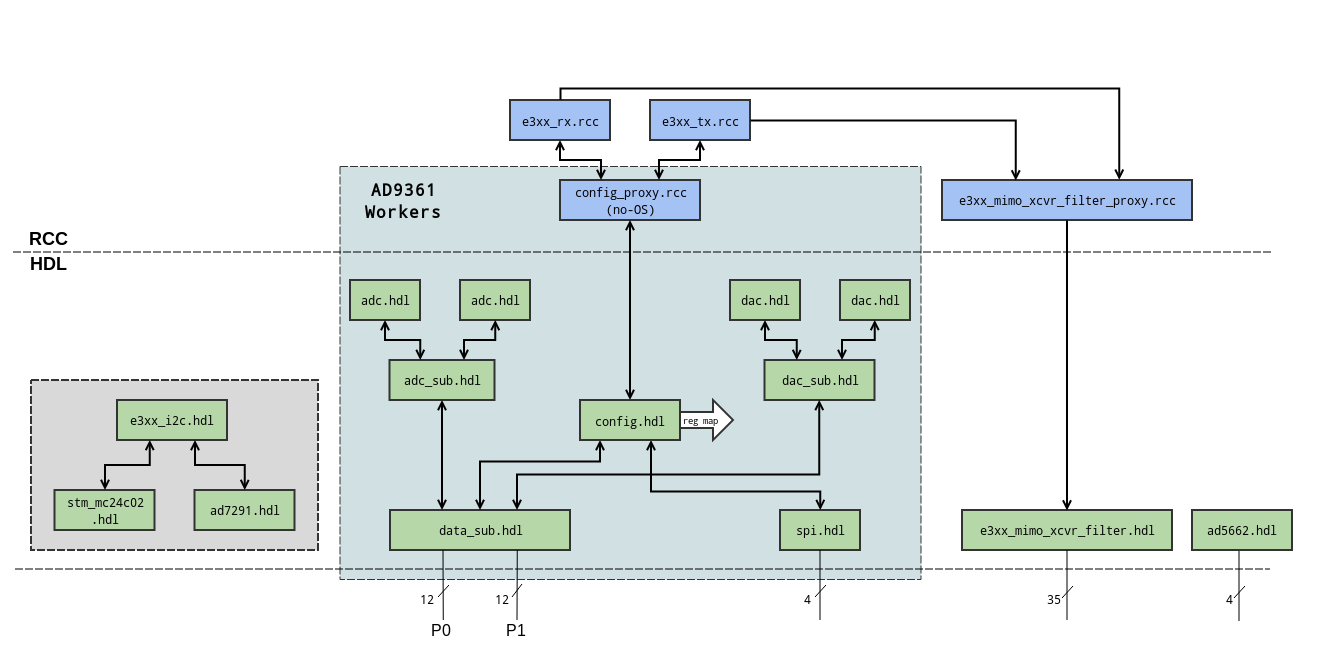
\includegraphics[scale=0.43]{E310_Workers}}
	\caption{E3XX Device Workers and Software Control Proxy Workers}
	\label{fig:wks}
\end{figure}

\begin{landscape}
The E3XX Platform Worker provides the device, proxy, and application workers with interfaces to the control and data planes as necessary. The Platform Worker also instantiates and connects to the time\_server worker. A block diagram of the full Board Support Package is shown below:
\begin{figure}[ht]
	\centerline{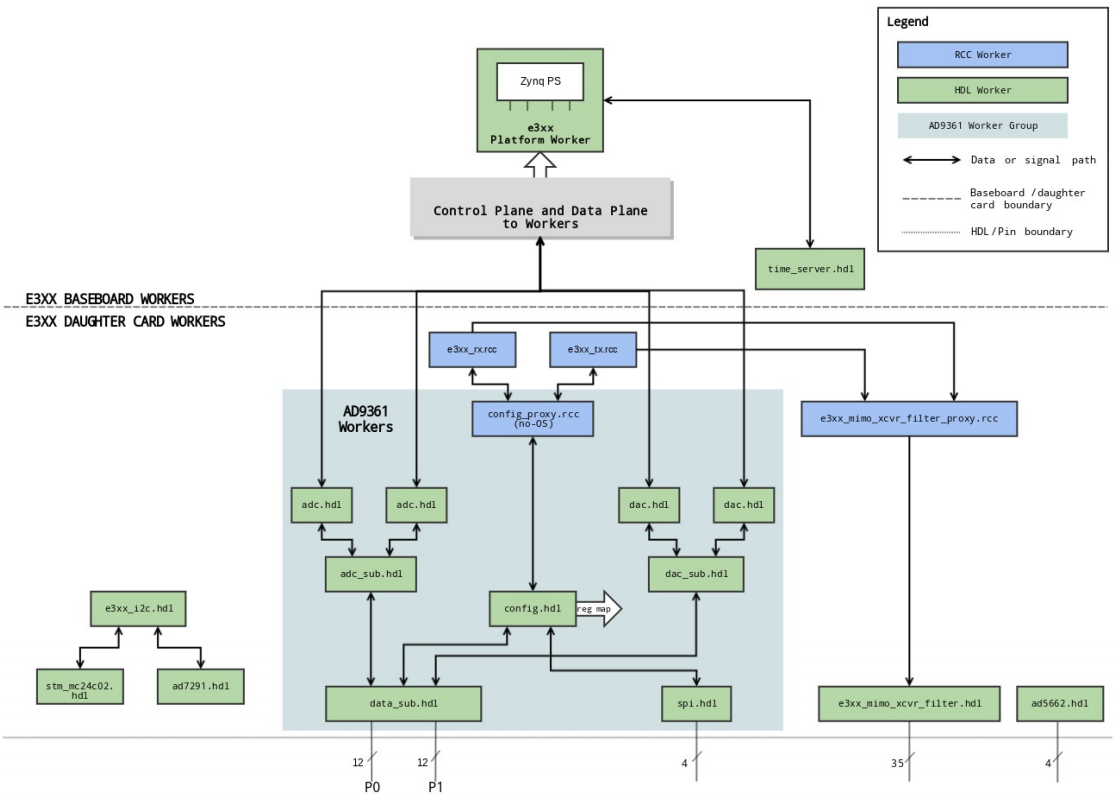
\includegraphics[scale=0.45]{E310_BSP}}
	\caption{E3XX BSP - Top Level Block Diagram}
	\label{fig:top}
\end{figure}
\end{landscape}
\end{flushleft}

\subsubsection*{Daughterboard}
\begin{flushleft}
This platform contains a daughterboard which is comprised of an AD9361 RF IC, an analog filter bank along with control signals, an AD5662 device, and an I2C device. Each of these has a device worker(s) and/or a software proxy for control. The AD9361 device workers are truly platform agnostic, and therefore were not developed specifically for the E310 radio. That being said, modifications were made to these device workers in order to support the E310 and its CMOS configurations in particular. More information on each of these devices and proxies can be found in each respective data sheet.

\end{flushleft}

\section*{Theory}
Because there are no data processing algorithms implemented in this worker, no corresponding data processing theory is relevant herein.

\section*{Block Diagrams}
\subsection*{Top level}
\makeatletter
\newcommand{\gettikzxy}[3]{%
  \tikz@scan@one@point\pgfutil@firstofone#1\relax
  \edef#2{\the\pgf@x}%
  \edef#3{\the\pgf@y}%
}
\makeatother
\pgfooclass{clientbox}{ % This is the class clientbox
    \method clientbox() { % The clientbox
    }
    \method apply(#1,#2,#3,#4) { % Causes the clientbox to be shown at coordinate (#1,#2) and named #3
        \node[rectangle,draw=white,fill=white] at (#1,#2) (#3) {#4};
    }
}
\pgfoonew \myclient=new clientbox()
\begin{center}
  \begin{tikzpicture}[% List of styles applied to all, to override specify on a case-by-case
      every node/.style={
        align=center,      % use this so that the "\\" for line break works
        minimum size=2cm,  % creates space above and below text in rectangle
        minimum width=4cm
      },
      every edge/.style={draw,thick}
    ]
    \node[rectangle,ultra thick,draw=black,fill=blue](R2){\Comp};
    \node[rectangle,draw=white,fill=white,minimum size=1.0cm](R5)[below= of R2]{timebase};
    \node[rectangle,draw=white,fill=white](placeholder)[above= of R2]{};
    \path[->]
    (R2)edge []  node [] {} (R5)
    (R5)edge []  node [] {} (R2)
    ;
    \gettikzxy{(placeholder)}{\rx}{\ry}
    \myclient.apply(\rx - 50,\ry,C1,\\ metadata);
    \path[<->]($(R2.north) + (-50 pt,0)$) edge [] node [] {} (C1);
    \myclient.apply(-\rx + 50,\ry,C1, ``zynq" \\ scalable data plane );
    \path[<->]($(R2.north) + (50 pt,0)$) edge [] node [] {} (C1);
    \myclient.apply(-\rx,\ry+50,C1, \\ cpmaster);
    \path[<->]($(R2.north) + (0 pt,0)$) edge [] node [] {} (C1);

  \end{tikzpicture}
\end{center}

\subsection*{State Machines}
Various state machines exist in the zynq, axi, and sdp primitive libraries. See primitive library source code for details. The explicit source code files included in the aforementioned primitives are enumerated in the following section.

\newpage
\section*{Source Dependencies}
\begin{itemize}
	\item
ocpi.bsp.e310/hdl/platforms/e3xx/e3xx.vhd
	\item
opencpi/hdl/primitives/zynq/zynq\_pkg.vhd
	\item
opencpi/hdl/primitives/zynq/zynq\_ps.vhd
	\item
opencpi/hdl/primitives/axi/axi\_pkg.vhd
	\item
opencpi/hdl/primitives/axi/axi2cp.vhd
	\item
opencpi/hdl/primitives/sdp/sdp2axi\_rd.vhd
	\item
opencpi/hdl/primitives/sdp/sdp2axi.vhd
	\item
opencpi/hdl/primitives/sdp/sdp2axi\_wd.vhd
	\item
opencpi/hdl/primitives/sdp/sdp\_axi\_pkg.vhd
	\item
opencpi/hdl/primitives/sdp/sdp\_pkg.vhd
	\item
opencpi/hdl/primitives/sdp/sdp\_body.vhd
\end{itemize}

\begin{landscape}
	\section*{Component Spec Properties}
	\begin{scriptsize}
		\begin{tabular}{|p{3cm}|p{1.5cm}|c|c|c|p{1.5cm}|p{1cm}|p{6cm}|}
			\hline
			\rowcolor{blue}
			Name               & Type   & SequenceLength & ArrayDimensions & Accessibility      & Valid Range & Default & Usage                                                                         \\
			\hline
			\verb+platform+    & String & 31             & -               & Parameter & Standard & - & Name of this platform                                                     \\
			\hline
			\verb+sdp_width+   & UChar  & -              & -               & Parameter & Standard & 1 & Width of data plane in DWORDS                                             \\
			\hline
			\verb+UUID+        & ULong  & -              & 16              & Readable           & Standard    & -       & UUID of this platform                                                         \\
			\hline
			\verb+oldtime+     & ULongLong & -           & -               & Padding            & Standard    & -       & N/A                                                                           \\
			\hline
			\verb+romAddr+     & UShort & -              & -               & Writable           & Standard    & -       &                                                                               \\
			\hline
			\verb+romData+     & ULong  & -              & -               & Volatile           & Standard    & -       &                                                                               \\
			\hline
			\verb+nSwitches+   & ULong  & -              & -               & Readable           & Standard    & -       & Number of switches                                                            \\
			\hline
			\verb+nLEDs+       & ULong  & -              & -               & Readable           & Standard    & -       & Number of LEDs                                                                 \\
			\hline
			\verb+memories_length+ & ULong & -           & -               & Readable           & Standard    & -       &                                                                               \\
			\hline
			\verb+memories+    & ULong  & -              & 4               & Readable           & Standard    & -       & The memory regions that may be used by \\
  	                     &        &                &                 &                    &             &         & various other elements, which          \\
  	                     &        &                &                 &                    &             &         & inidicates aliasing etc.               \\
                         &        &                &                 &                    &             &         & The values describing each region are: \\
                         &        &                &                 &                    &             &         & Bit 31:28 - External bus/BAR connected \\
                         &        &                &                 &                    &             &         &             to this memory (0 is none) \\
                         &        &                &                 &                    &             &         & Bit 27:14 - Offset in bus/BAR of this  \\
                         &        &                &                 &                    &             &         &             memory (4KB units)         \\
                         &        &                &                 &                    &             &         & Bit  13:0 - Size of this memory (4KB units) \\
                         &        &                &                 &                    &             &         &             units) \\
			\hline
			\verb+dna+         & ULongLong & -           & -               & Readable           & Standard    & -       & DNA (unique chip serial number) of this platform \\
			\hline
			\verb+switches+    & ULong  & -              & -               & Volatile           & Standard    & -       & Current value of any switches in the platform                                 \\
			\hline
			\verb+LEDS+        & ULong  & -              & -               & Writable, Readable & Standard    & -       & Setting of LEDs in the platform, with readback                                \\
			\hline
			\verb+nSlots+      & ULong  & -              & -               & Parameter & Standard & 0 & Number of slots available for cards, which indicates the usable length of the slotCardIsPresent array property. \\
			\hline
			\verb+slotNames+   & String & 32             & -               & Parameter & Standard & "" & A string which is intended to include comma-separated names of the slots available for cards. The inter-comma position of each name corresponds to the same index of the slotCardIsPresent array property. \\
			\hline
			\verb+slotCardIsPresent+ & Bool & -          & 64              & Volatile           & Standard    & -       & An array of booleans, where each index contains an indication whether a card is physically present in the given index's slot. For a description of a given index's slot, see the corresponding comma-separated string contents in the slotName property. Note that only the first min(nSlots,64) of the 64 indices contain pertinent information. \\
			\hline

		\end{tabular}
	\end{scriptsize}
	\section*{Worker Properties}
	\begin{scriptsize}
		\begin{tabular}{|p{1.5cm}|p{2.5cm}|p{1.5cm}|c|c|c|p{2cm}|p{1.1cm}|p{4cm}|}
			\hline
			\rowcolor{blue}
			Property Type & Name                  & Data Type  & SequenceLength & ArrayDimensions & Accessibility       & Valid Range & Default & Usage                        \\
			\hline
			SpecProperty & \verb+platform+       & String & 31            & -               & Parameter           & Standard    & e3xx & Name of this platform  \\
			\hline
			SpecProperty & \verb+nSlots+         & ULong  & -             & -               & Parameter & Standard & 1 & Number of slots available for cards, which indicates the usable length of the slotCardIsPresent array property. \\
			\hline
			SpecProperty & \verb+slotNames+      & String & 32            & -               & Parameter & Standard & e3xx\_conn & A string which is intended to include comma-separated names of the slots available for cards. The inter-comma position of each name corresponds to the same index of the slotCardIsPresent array property. \\
			\hline

			Property     & \verb+useGP1+         & Bool   & -             & -               & Parameter           & Standard    & false   &                              \\
			\hline
			Property     & \verb+axi_error+      & Bool   & -             & 4               & Volatile            & Standard    & -       &                              \\
			\hline
			Property     & \verb+sdpDropCount+   & UChar  & -             & -               & Volatile            & Standard    & -       &                              \\
			\hline
			Property     & \verb+debug_state+    & ULongLong & -          & 4               & Volatile            & Standard    & -       &                              \\
			\hline
			Property     & \verb+debug_state1+   & ULongLong & -          & 4               & Volatile            & Standard    & -       &                              \\
			\hline
			Property     & \verb+debug_state2+   & ULongLong & -          & 4               & Volatile            & Standard    & -       &                              \\
			\hline
			Property     & \verb+onswitch_db_p+  & Bool  & -              & -               & Volatile            & Standard    & -       & Property required to force a pull-up on the ON\_SWITCH\_DB pin. This is required because the compilation tools seem to otherwise optimize out the pull-up.\\
			\hline
		\end{tabular}
	\end{scriptsize}

	\section*{Component Ports}
	No ports are implemented for the given component specification.

	\section*{Worker Interfaces}
	\begin{scriptsize}
		\begin{tabular}{|M{2cm}|M{2cm}|M{1.5cm}|M{1.5cm}|M{14.5cm}|}
			\hline
			\rowcolor{blue}
			Type       & Name & Master & Count & Usage                  \\
			\hline
			metadata   & -    & true   & -     & Access to container metadata via the platform worker. All platform workers must provide this port. \\
			\hline
			timebase   & -    & true   & -     & Providing a timebase for the time service. All platform workers must provide this port. \\
			\hline
			cpmaster   & -    & true   & -     & This platform worker provides a control plane. \\
			\hline
			sdp        & zynq & true   & 4     & Scalable data plane. \\
			\hline
		\end{tabular}
	\end{scriptsize}

\end{landscape}
\pagebreak
	\section*{Worker Devices}
	The following is a table which enumerates which device workers are allowed in platform configurations and in assembly containers. The parameter values specify restricted/allowed implementations. Note that the worker signals listed are only those who are unconnected on the platform or whose platform signal name differ from the worker signal name. Note that device workers allowed by cards are not included in this list.\\
			\begin{tabular}{|M{3cm}|M{3.5cm}|M{3cm}|M{3cm}|M{3cm}|}
			\hline
			\rowcolor{blue}
			Name                       & Property Name    & Property Value              & Worker Signal & Platform Signal         \\
			\hline
			time\_server               & frequency        & 100*10\textsuperscript{6}   &               &                         \\
			\hline
		\end{tabular}
	\section*{Worker Devices on E3XX MIMO XCVR Card}
	The following is a table which enumerates which device workers are allowed in platform configurations and in assembly containers. The parameter values specify restricted/allowed implementations. Note that the worker signals listed are only those who are unconnected on the platform or whose platform signal name differ from the worker signal name. Note that device workers allowed by cards are not included in this list.\\
			\begin{tabular}{|M{3.5cm}|M{3.5cm}|M{2.5cm}|M{3cm}|M{3cm}|}
			\hline
			\rowcolor{blue}
			Name                       & Property Name      & Property Value              & Worker Signal & Platform Signal         \\
			\hline
			e3xx\_mimo\_xcvr\_ad5662 &                    &                             & -             & -                       \\			
			\hline
			e3xx\_i2c                  &                    &                             & -             & -                       \\
			\hline
			e3xx\_mimo\_xcvr\_filter   &                    &                             & -             & -                       \\
			\hline
			ad9361\_spi                &CP\_CLK\_FREQ\_HZ\_p& 100e6                       & -             & -                       \\
			\hline
			ad9361\_config             &                    &                             & -             & -                       \\
			\hline
      \multirow{8}{*}{ad9361\_data\_sub} &lvds\_p   & false                       & -             & -                       \\ 
                                 &half\_duplex\_p   & false                       & -             & -                       \\ 
                                 &single\_port\_p   & true                        & -             & -                       \\ 
                                 &swap\_ports\_p    & false (true also supported) & -             & -                       \\ 
                                 &DATA\_CLK\_Delay  & 11                          & -             & -                       \\
                                 &RX\_Data\_Delay   & 0                           & -             & -                       \\
                                 &FB\_CLK\_Delay    & 3                           & -             & -                       \\
                                 &TX\_Data\_Delay   & 0                           & -             & -                       \\                                 
			\hline
      \multirow{3}{*}{ad9361\_adc\_sub} &lvds\_p    & false                       & -             & -                       \\ 
                                 &half\_duplex\_p   & false                       & -             & -                       \\ 
                                 &single\_port\_p   & true                        & -             & -                       \\                         
			\hline
      \multirow{3}{*}{ad9361\_dac\_sub} &lvds\_p    & false                       & -             & -                       \\ 
                                 &half\_duplex\_p   & false                       & -             & -                       \\ 
                                 &single\_port\_p   & true                        & -             & -                       \\                        
			\hline
      		ad9361\_adc0\textsuperscript{\ref{adcnumpresent}}  & -    & -                           & -             & -                       \\ 
			\hline
      		ad9361\_dac0\textsuperscript{\ref{adcnumpresent}} & -    & -                           & -             & -                       \\ 
			\hline
      		ad9361\_adc1\textsuperscript{\ref{adcnumpresent}} & -    & -                           & -             & -                       \\ 
			\hline
			ad9361\_dac1\textsuperscript{\ref{adcnumpresent}} & -    & -                           & -             & -                       \\ 
			\hline
		\end{tabular}
		\footnotetext[1]{\label{adcnumpresent}Depending on the mode (0rx1tx,1rx0tx,1rxtx...2rx2tx), there may be between 0 and 2 ad9361\_adc/dac workers in the platform configuration.}
\section*{Signals}
Note that this signal table does not include signals that may be provided by slots. \\
\begin{tabular}{|c|c|c|c|p{8cm}|}
	\hline
	\rowcolor{blue}
	Name           & Type   & Differential & Width & Description                                          \\
	\hline
	PPS\_EXT\_IN & Output & false        & 1     & Connected to time\_server. Requires external connection. Note that the timer\_server has not been thoroughly tested on this system.\\
	\hline
	ONSWITCH\_DB    & Input & false        & 1     & Onswitch pin to be debounced - tied to pull-up and a volatile property. This is needed in order to enforce that the onswitch is tied to a pull-up, or the radio reboots when the bitstream is loaded. The volatile property forces the compilation tools \textit{not} to optimize the signal and pull-up out.\\
	\hline
\end{tabular}
\pagebreak
\section*{Slots}
The following table enumerates the available slots for this platform and the signals they include. Note that the signals listed are only those who are unconnected on the platform or whose platform signal name do not match the slot signal name. \\
\begin{longtable}[l]{|c|c|c|c|}
	\hline
	\rowcolor{blue}
	Name           & Type & Slot Signal & Platform Signal  \\
	\hline
	E3XX\_CONN & e3xx\_conn & - & - \\
	\hline
\end{longtable}
\section*{Platform Configurations}
	\begin{tabular}{|c|c|c|c|}
		\hline
		\rowcolor{blue}
		Name & Platform Configuration Workers & Card & Slot \\
		\hline
		\multirow{2}{*}{base} &\comp & - & - \\ &time\_server & - & - \\
		\hline
		\multirow{9}{*}{cfg\_[0$|$1$|$2]rx\_[0$|$1$|$2]tx\_mode\_[2$|$3]} &\comp & - & - \\ &time\_server & - & - \\ &e3xx\_mimo\_xcvr\_ad5662& - & - \\ &e3xx\_mimo\_xcvr\_filter & - & - \\ &e3xx\_i2c & - & - \\ &ad9361\_spi & - & - \\ &ad9361\_data\_sub & - & - \\ &ad9361\_config & - & - \\ &ad9361\_adc\_sub & - & - \\ &ad9361\_dac\_sub & - & - \\ &ad9361\_adc\textsuperscript{\ref{adcnumpresent}} & - & - \\ &ad9361\_dac\textsuperscript{\ref{adcnumpresent}} & - & - \\
		\hline
	\end{tabular}
\footnotetext[1]{\label{adcnumpresent}Depending on the mode (0rx1tx,1rx0tx,1rxtx...2rx2tx), there may be between 0 and 2 ad9361\_adc/dac workers in the platform configuration.}
\section*{Control Timing and Signals}
\subsection*{Control Domain}
All control clocking in the E3XX platform originates from the PS7 processing clock 0 (FCLK0), which is set to 100 MHz.

\subsection*{Sampling Domain}
The sampling clock domain originates from the AD9361's DATA\_CLK\_P output. It is labeled CAT\_DATA\_CLK on the daughterboard connector, and is ultimately assigned to the E3XX\_CONN\_CAT\_DATA\_CLK input pin in the constraints file. This clock is routed to the AD9361 device workers (specifically ad9361\_data\_sub.hdl) via OpenCPI card/slot constructs.\par\medskip
\noindent This clock is used by the ad9361\_adc\_sub.hdl and ad9361\_dac\_sub.hdl workers. Additionally, the ad9361\_dac\_sub.hdl generates FB\_CLK, which is routed through the card/slot to the E3XX\_CONN\_CAT\_FB\_CLK output pin in the constraints file. This clock is transmitted alongside TX data in a source synchronous fashion. See the AD9361 device worker documentation and ADI's UG-570 for more information regarding the relationships between these clocks.

\section*{Performance and Resource Utilization}
\todo{Update tables with final utilization}
\subsection*{E3xx `Base' Configuration}
\begin{scriptsize}
	\begin{tabular}{|c|c|c|c|c|c|}
		\hline
		\rowcolor{blue}
		Device                & Registers & LUTs & Fmax        & Memory/Special Functions & Design Suite \\
		\hline
		Zynq XC7Z020-1-CLG484 & 2290      & 2702 & 173.973 MHz & N/A                      & Vivado 2017.1    \\
		\hline
	\end{tabular}
\end{scriptsize}

\subsection*{E3xx `1rx0tx\_mode\_2' Configuration (CMOS Single Port Full Duplex)}
\begin{scriptsize}
	\begin{tabular}{|c|c|c|c|c|c|c|c|}
		\hline
		\rowcolor{blue}
		Device                & Registers & LUTs & Fmax        & Memory/Special Functions & Design Suite \\
		\hline
		Zynq XC7Z020-1-CLG484 & 2960      & 3775 & 173.973 MHz & N/A                      & Vivado 2017.1    \\
		\hline
	\end{tabular}
\end{scriptsize}

\subsection*{E3xx `0rx1tx\_mode\_2' Configuration (CMOS Single Port Full Duplex)}
\begin{scriptsize}
	\begin{tabular}{|c|c|c|c|c|c|c|c|}
		\hline
		\rowcolor{blue}
		Device                & Registers & LUTs & Fmax        & Memory/Special Functions & Design Suite \\
		\hline
		Zynq XC7Z020-1-CLG484 & 2960      & 3775 & 173.973 MHz & N/A                      & Vivado 2017.1    \\
		\hline
	\end{tabular}
\end{scriptsize}

\subsection*{E3xx `1rx1tx\_mode\_2' Configuration (CMOS Single Port Full Duplex)}
\begin{scriptsize}
	\begin{tabular}{|c|c|c|c|c|c|c|c|}
		\hline
		\rowcolor{blue}
		Device                & Registers & LUTs & Fmax        & Memory/Special Functions & Design Suite \\
		\hline
		Zynq XC7Z020-1-CLG484 & 2960      & 3775 & 173.973 MHz & N/A                      & Vivado 2017.1    \\
		\hline
	\end{tabular}
\end{scriptsize}

\subsection*{E3xx `2rx2tx\_mode\_2' Configuration (CMOS Single Port Full Duplex)}
\begin{scriptsize}
	\begin{tabular}{|c|c|c|c|c|c|c|c|}
		\hline
		\rowcolor{blue}
		Device                & Registers & LUTs & Fmax        & Memory/Special Functions & Design Suite \\
		\hline
		Zynq XC7Z020-1-CLG484 & 2960      & 3775 & 173.973 MHz & N/A                      & Vivado 2017.1    \\
		\hline
	\end{tabular}
\end{scriptsize}\\

\noindent Note that there are many possible configurations of this platform. For each combination of CMOS Single/Dual Port, Half/Full Duplex and ports-swapped/not swapped, there is also a 0rx1tx, 1rx0tx, 1rx1tx, ... 2rx2tx. The resource utilization is only listed here for some of these, but can be extracted from the synthesized platform configuration for the supported modes. For now, the only supported modes are those corresponding to CMOS Single Port Full Duplex.
\section*{Test and Verification}
\noindent Testing performed to verify functionality of the Platform Worker includes running of basic unit/application tests to test the Platform Worker itself, as well as device worker unit tests and system level application tests. \\

\noindent To test the basic functionality of the Platform Worker, simple applications such as \code{testbias} and unit tests such as \code{bias.test} were executed. These verify the basic functionality of the Platform Worker and its communication with the \code{xilinx13\_4} Software Platform. \\

\noindent To further test the Platform Worker's functionality paired with its device workers, device worker unit tests were modified and performed for the AD9361 device workers, the E3XX XCVR Filter device worker and proxy, the AD5662 device worker, and the RX and TX proxy workers. Each of these tests has its own document that can be reviewed for further information. \\

\noindent Finally, OpenCPI reference applications were modified and tested on the E310 radio using the AD9361 workers in CMOS Single Port Full Duplex DDR mode. This provides a full system test along the RX and TX paths.

\end{document}
